\subsection{Microservices Architecture}

\subsubsection{Mô tả hệ thống}
Microservices Architecture phân rã hệ thống IoT thành một tập hợp các đơn vị Independent Services với cơ chế Loose Coupling. Thay vì một khối mã nguồn duy nhất, hệ thống được module hóa dựa trên các phạm vi nghiệp vụ cụ thể như: Quản trị thiết bị, Thu nhận dữ liệu cảm biến, hoặc Xử lý sự kiện cảnh báo.

Đặc điểm cốt lõi của mô hình này nằm ở tính cô lập về dữ liệu và thực thi, mỗi dịch vụ toàn quyền quản lý cơ sở dữ liệu riêng biệt, giúp tránh tình trạng phụ thuộc chéo ở tầng lưu trữ. Việc trao đổi thông tin giữa các dịch vụ được thực hiện thông qua các API sử dụng giao thức mạng như REST, gRPC hoặc các hệ thống trung gian truyền tin (Message Broker) để đảm bảo tính phi tập trung của toàn hệ thống.

\paragraph*{Sơ đồ kiến trúc}

\begin{figure}[H]
    \centering
    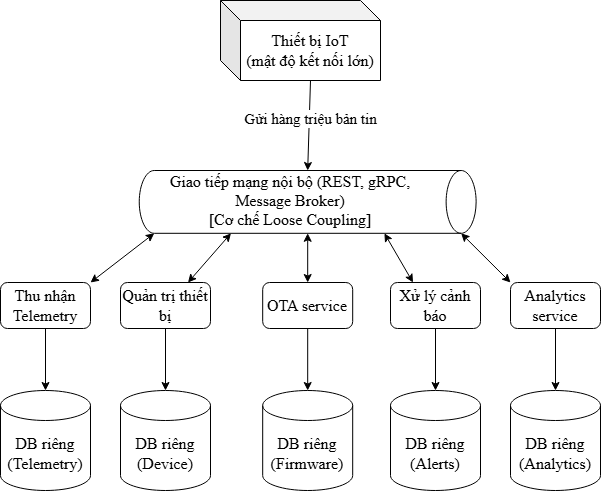
\includegraphics[width=0.9\linewidth]{graphics/MicroservicesArchitecture.drawio.png}
    \caption{Microservices Architecture}
    \label{fig:microservices_architecture}
\end{figure}

\subsubsection{Phân tích sự đánh đổi}
Việc chuyển đổi sang Microservices là một quyết định đánh đổi chiến lược, tập trung vào việc tối ưu hóa Elasticity và tính ổn định của hệ thống trên quy mô lớn. Ở khía cạnh lợi thế, kiến trúc này cung cấp Granular Scalability, cho phép điều phối tài nguyên độc lập dựa trên tải thực tế của từng dịch vụ. Điển hình là việc tăng cường năng lực xử lý cho tầng Telemetry Ingestion để tiếp nhận hàng triệu bản tin mà không gây lãng phí tài nguyên cho các dịch vụ có tần suất hoạt động thấp như OTA.

Song song đó, Fault Isolation giúp khu trú các sự cố tại một điểm (như dịch vụ Analytics) để ngăn chặn hiện tượng sụp đổ dây chuyền, mặc dù điều này đòi hỏi việc triển khai thêm các mẫu thiết kế phức tạp như Circuit Breaker hoặc Bulkhead để kiểm soát luồng thực thi.

Tuy nhiên, những ưu thế trên đi kèm với sự gia tăng đáng kể về Operational Complexity và các rào cản về hiệu năng. Hệ thống yêu cầu một hạ tầng quản trị tinh vi bao gồm Kubernetes, Service Mesh và Distributed Tracing, dẫn đến việc tiêu tốn một phần lớn nguồn lực kỹ thuật (ước tính từ $40\%$ đến $60\%$) cho công tác duy trì hạ tầng thay vì tập trung vào phát triển logic nghiệp vụ.

Bên cạnh gánh nặng về quản trị, Inter-service Latency phát sinh từ các bước Network hops giữa các dịch vụ cũng là một tham số kỹ thuật trọng yếu. Với độ trễ tích lũy dao động từ 10-30ms cho mỗi giao tiếp nội bộ, việc duy trì tổng thời gian phản hồi dưới 100ms trong các ứng dụng điều khiển IoT thời gian thực trở thành một thách thức lớn, đòi hỏi các giải pháp tối ưu hóa mạng hoặc chuyển đổi giao thức liên lạc một cách thận trọng.

Bảng \ref{tab:microservices-tradeoffs} dưới đây đúc kết các ưu điểm và hạn chế cốt lõi của mô hình Microservices Architecture nhằm cung cấp cái nhìn tổng quan về khả năng vận hành của hệ thống.

\begin{table}[H]
\centering
\caption{Trade-off của Microservices Architecture trong IoT}
\label{tab:microservices-tradeoffs}
\begin{tabular}{|p{3.5cm}|p{5.5cm}|p{5.5cm}|}
\hline
\textbf{Tiêu chí} & \textbf{Ưu điểm} & \textbf{Nhược điểm} \\ \hline
\textbf{Tính mở rộng} & Cung cấp Granular Scalability, cho phép mở rộng độc lập các dịch vụ có tải cao (như Telemetry Ingestion) mà không gây lãng phí tài nguyên. & Cần hạ tầng mạng và định tuyến phức tạp để hỗ trợ việc co giãn liên tục của các dịch vụ. \\ \hline
\textbf{Tính ổn định \& Cô lập lỗi} & Tính năng Fault Isolation giúp khu trú sự cố tại một điểm (vd: dịch vụ Analytics sập), ngăn chặn hiện tượng sụp đổ dây chuyền. & Phải triển khai thêm các mẫu thiết kế kiểm soát luồng phức tạp như Circuit Breaker hoặc Bulkhead. \\ \hline
\textbf{Độ phức tạp vận hành} & Tối ưu hóa Elasticity và tính ổn định của hệ thống trên quy mô lớn, hỗ trợ các đội ngũ độc lập làm việc song song. & Gia tăng đáng kể Operational Complexity. Tiêu tốn 40\%-60\% nguồn lực kỹ thuật chỉ để duy trì hạ tầng tinh vi (Kubernetes, Service Mesh, Tracing). \\ \hline
\textbf{Hiệu năng \& Latency} & Dịch vụ được phân rã giúp tối ưu hóa xử lý cho từng phạm vi nghiệp vụ cụ thể. & Phát sinh Inter-service Latency do Network hops (10-30ms/giao tiếp), gây thách thức lớn cho các ứng dụng IoT thời gian thực cần độ trễ dưới 100ms. \\ \hline
\end{tabular}
\end{table}

\subsubsection{Ngữ cảnh áp dụng và Ngưỡng tới hạn}
Hiệu quả thực thi của Microservices Architecture tỷ lệ thuận với quy mô thiết bị và năng lực quản trị vận hành của tổ chức. Kiến trúc này đạt đến trạng thái tối ưu trong các hệ sinh thái IoT công nghiệp có mật độ kết nối lớn (vượt ngưỡng $10.000$ thiết bị), nơi yêu cầu về sự phân rã dịch vụ trở nên cấp thiết để hỗ trợ các đội ngũ phát triển độc lập làm việc song song.

Ngược lại, mô hình này được xem là một lựa chọn không phù hợp đối với các doanh nghiệp khởi nghiệp ở giai đoạn sơ khởi, các nhóm kỹ thuật tinh gọn dưới $5$ nhân sự, hoặc những ứng dụng đặc thù yêu cầu độ trễ phản hồi cực thấp dưới ngưỡng $10ms$. Trong những kịch bản quy mô nhỏ hoặc yêu cầu thời gian thực khắt khe, gánh nặng về chi phí duy trì hạ tầng và độ trễ phát sinh từ giao tiếp mạng nội bộ sẽ triệt tiêu hoàn toàn các lợi ích về khả năng mở rộng, tạo ra một rào cản lớn đối với mục tiêu tối ưu hóa tài nguyên và tốc độ phân phối sản phẩm.

\subsubsection{Summary}
Tóm lại, Microservices Architecture là một giải pháp kiến trúc mang tính chiến lược nhằm giải quyết bài toán về quy mô và tính ổn định cho các hệ thống IoT phức tạp. Mặc dù cung cấp khả năng co giãn linh hoạt và cô lập lỗi hiệu quả, kiến trúc này đòi hỏi một sự đánh đổi nghiêm ngặt về hiệu năng mạng và nguồn lực vận hành hạ tầng. Việc quyết định áp dụng Microservices không chỉ đơn thuần là một lựa chọn kỹ thuật, mà còn là sự cân nhắc về mức độ trưởng thành của đội ngũ và yêu cầu đặc thù về độ trễ của hệ thống đích.